\documentclass[12pt,a4paper]{report}

% Paquetes básicos
\usepackage[utf8]{inputenc}
\usepackage[spanish,es-tabla]{babel} % Idioma español
\usepackage{graphicx} % Para insertar imágenes
\usepackage{geometry} % Configuración de márgenes
\usepackage{setspace} % Interlineado
\usepackage{lipsum} % Texto de relleno (puedes borrarlo)

% Configuración de márgenes
\geometry{
    left=3cm,
    right=2.5cm,
    top=2.5cm,
    bottom=2.5cm
}

\begin{document}

% ------------------- PORTADA -------------------
\begin{titlepage}
    % Para que la imagen ocupe todo el ancho sin respetar márgenes, usamos un truco con \hspace
    \noindent\makebox[\textwidth][c]{%
        % Reemplaza 'uo-big.png' con el nombre real de tu imagen.
        % height=0.45\textheight asegura que ocupe un poco menos de la mitad de la página.
        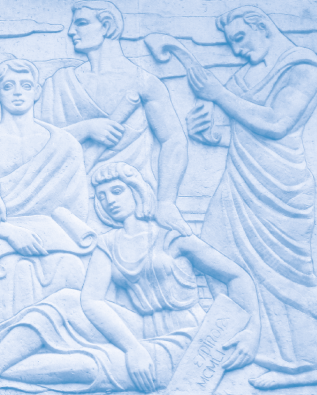
\includegraphics[width=\paperwidth,height=0.45\textheight,keepaspectratio=false]{uo-big.png}
    }
    
    \vspace{2cm} % Espacio entre la imagen y el texto
    
    \begin{center}
        {\LARGE \textbf{FACULTAD DE CIENCIAS NATURALES Y EXACTAS}} \\[1cm]
        {\Large \textbf{DEPARTAMENTO DE CIENCIAS DE LA COMPUTACIÓN}} \\[2.5cm]
        
        {\Huge \textbf{Título de tu Proyecto o Paper}} \\[2.5cm]
        
        {\Large \textbf{Autora:}} \\
        {\Large [Tu Nombre Aquí]} \\[2cm]
        
        \vfill
        
        {\large \today}
    \end{center}
\end{titlepage}
% -----------------------------------------------

\doublespacing % Interlineado doble, común en proyectos académicos

% ------------------- RESUMEN Y ABSTRACT -------------------
\chapter*{Resumen}
\addcontentsline{toc}{chapter}{Resumen}
Aquí va el resumen de tu trabajo en español. Debe ser conciso y explicar el problema, la metodología y los resultados principales.

\vspace{1cm}

\textbf{Palabras clave:} LaTeX, Plantilla, Universidad, Proyecto.

\chapter*{Abstract}
\addcontentsline{toc}{chapter}{Abstract}
Here goes the abstract of your work in English. It should be concise and explain the problem, methodology, and main results.

\vspace{1cm}

\textbf{Keywords:} LaTeX, Template, University, Project.
% ---------------------------------------------------------

% ------------------- ÍNDICE -------------------
\tableofcontents
\newpage
% ----------------------------------------------


% ------------------- DESARROLLO -------------------
\chapter{Desarrollo}
Este es el primer capítulo de desarrollo. Puedes dividirlo en secciones según lo necesites.

\section{Introducción al problema}
Aquí puedes comenzar a escribir el contenido de tu investigación.

\subsection{Subsección de ejemplo}
Si necesitas más jerarquía, usa subsecciones.

% --------------------------------------------------

% ------------------- CONCLUSIONES -------------------
\chapter{Conclusiones}
En este capítulo presentarás las conclusiones de tu trabajo, basadas en los resultados obtenidos durante el desarrollo.
% ----------------------------------------------------

% ------------------- BIBLIOGRAFÍA -------------------
% Usaremos el entorno thebibliography para algo sencillo. 
% Si necesitas algo más complejo, puedes investigar sobre BibTeX o Biber.
\renewcommand{\bibname}{Bibliografía}
\begin{thebibliography}{99}
\addcontentsline{toc}{chapter}{Bibliografía}

\bibitem{referencia1} 
Apellido, Nombre. \textit{Título del libro o paper}. Editorial o Revista, Año.

\end{thebibliography}
% ----------------------------------------------------

\end{document}
